%!TEX root = aaai2014.tex
\section{METHOD}
\label{sec:method}

In the subsequent analysis, we assume that a trainer provides feedback for the actions taken by a learner. Specifically, we consider the user is delivering signals that can be mapped into binary feedback: correct $c$ and incorrect $w$. 

\subsection{World and Task}
We consider a 5x5 grid world, where an agent can perform five different discrete actions: move up, down, left, right, or a ``no move'' action. The user goal is to teach the agent to reach one (unknown to the agent) of the $25$ discrete positions which represent the set of possible tasks. We thus consider that the agent has access to 25 different task hypothesis (one with goal location at each of the cells). We use \textit{Markov Decision Processes} (MDP) to represent the problem \cite{sutton1998reinforcement}. From a given task $\xi$, represented as a reward function, we can compute the corresponding policy $\pi^{\xi}$ using, for instance, Value Iteration \cite{sutton1998reinforcement}. The policies allow us to interpret the teaching signals with respect to the interaction protocol defined. For the current work we will consider the user is providing feedback on the agent action. We define $p(l | s, a, \xi)$ as:
%
\begin{equation*}
    p(l | s, a, \xi) = 
    \begin{cases}
	1-\alpha               & if~a = \argmax_a \pi^{\xi}(s,a)\\
        \alpha             & \text{otherwise}\\
   \end{cases}
\end{equation*}
with $\alpha$ modeling the expected error rate of the user. 
% We use $\alpha = 0.1$.

\subsection{Signal properties and classifier}

We aim at applying this algorithm to error-related potentials (ErrPs) for EEG-based BCI applications. These signals are generated in the user's brain after s/he assesses actions performed by an external agent \cite{chavarriaga2010learning}, where correct and erroneous assessments will elicit different brain signals. Past approaches have already demonstrated that these signals can be classified online with accuracies of around 80\% and translated into binary feedback, thanks to a prior calibration session that lasts for 30-40 minutes \cite{chavarriaga2010learning, iturrate2013task}.

Following the literature \cite{blankertz2010single}, we will model the signals using independent multivariate normal distributions for each class, $\mathcal{N}(\mu_c, \Sigma_c), \mathcal{N}(\mu_w, \Sigma_w)$. With $\theta$ the set of parameters $\{\mu_c, \Sigma_c,\mu_w, \Sigma_w\}$. Given the high dimensionality of the problem we will also need to regularize. For this we apply shrinkage to the covariance matrix ($\lambda = 0.5$) and compute the value of the marginal pdf function using a noninformative (Jeffrey’s) prior [\cite{gelman2003bayesian}, p88]:
%
\begin{eqnarray}
p(e|l, \theta) & = & t_{n-d}(e | \mu_l,\frac{\Sigma_l (n+1)}{n(n-d)})
\label{eq:prior}
\end{eqnarray}
where $\theta$ represents the ML estimates (mean $\mu_l$ and covariance $\Sigma_l$ for each class $l$) required to estimate the marginal under the Jeffreys prior, $n$ is the number of signals, and $d$ is the dimensionality of a signal feature vector.

% \todo{$\theta$ in Eq. (10) abuses notation as it represents the ML estimates of previous data required to estimate the marginal under the Jeffreys prior. It will be changed to avoid confusion. However it remains the same idea, $\theta$ is representing a classifier.}


% Finally we compute the probability of a label given a signal:

% \begin{eqnarray}
% p(l^{\theta} = l | e, \theta) & = & \frac{p(e|l^{\theta} = l, \theta) p(l^{\theta} = l)}{\sum_{k \in {1, \ldots, L}} p(e|l^{\theta} = k, \theta) p(l^{\theta} = k)} \nonumber \\
% \end{eqnarray}
% with no apriori on the label $\forall l,  p(l^{\theta} = l) = \frac{1}{L}$ and from \cite{gelman2003bayesian}:
% \begin{eqnarray}
% p(e|l^{\theta} = l, \theta) & = & t_{n-d}(e | \mu_l,\frac{\Sigma_l (n+1)}{n(n-d)})
% \label{eq:prior}
% \end{eqnarray}
% where $n$ is the number of signal, $d$ is the dimensionality, $\mu_l$ and $\Sigma_l$ the mean and covariance of the multivariate normal distribution of class $l$.

% The predictions are finally corrected using the method described in section \ref{sec:algorithm}.


\subsection{Task Achievement}

A task is considered completed when the confidence level $\beta$ as been reached for this task and the agent is located at the task associated goal state. If the state is the one intended by the user it is a success. Whatever the success or failure of the first task, the user selects a new goal state randomly, the agent resets task likelihoods, propagates the believed labels, and teaching starts again. At no point the agent has access to a measure of its performance, it can only refer to the unlabeled feedback signals from the user.

\subsection{Evaluation scenarios}

Two different evaluation scenarios were tested with two different types of signals: artificial datasets, and real ErrP datasets recorded from previous experiments \cite{iturrate2013task}.

\paragraph{Artificial datasets}
The goal of this evaluation was to analyze the feasibility of learning a task from scratch in a 5x5 grid world. 
%
The artificial dataset was composed of two classes, with 1000 examples per class. Each example was generated by sampling from a normal distribution with a covariance matrix of diagonal 1 and mean selected randomly. The datasets were generated while varying two factors: (i) the dimensionality of the data, where 2, 5, 10 and 30 features were tested; and (ii) the quality of the dataset, measured in terms of the ten-fold accuracy the classifier would obtain. 

Once the datasets were generated, two different evaluations were performed: (i) the goodness of our proposed planning strategy versus a) random action selection, b) greedy action selection, and c) a task-only uncertainty based method; (ii) the time required by the agent to learn the first task (i.e. to reach the first target), and (iii) the number of tasks that can be learned in 500 iterations.

\paragraph{EEG datasets}
Once the algorithm was evaluated with artificial datasets, we tested the feasibility of the proposed self-calibration approach using real ErrP datasets. The objective of this analysis is to study the scalability of our method to EEG data, which may have different properties than our artificial dataset. 

The EEG data were recorded in a previous study \cite{iturrate2013task} where participants monitored on a screen the execution of a task where a virtual device had to reach a given goal. The motion of the device could be correct (towards the goal) or erroneous (away from the goal). The subjects were asked to mentally assess the device movements as erroneous or non-erroneous. The EEG signals were recorded with a gTec system with 32 electrodes distributed according to an extended 10/20 international system with the ground on FPz and the reference on the left earlobe. The ErrP features were extracted from two fronto-central channels (FCz and Cz) within a time window of $[200,700]$ ms (being 0 ms the action onset of the agent) and downsampled to $32$ Hz. This leaded to a vector of $34$ features.

\paragraph{Comparison with calibration methods}
In order to show the benefit of learning without explicit calibration, we compare our method with the standard supervised BCI calibration procedure. In this calibration procedure, which can last for up to 40 minutes, the experimenter needs to record enough data from the user from several offline runs, where the user is not controlling the agent but just passively assessing its actions.
%
Following the literature on ErrPs \cite{chavarriaga2010learning,iturrate2013task} our training data will consist of 80 percent of positive examples (associated to a correct feedback) and 20 percent of negative examples (associated to an incorrect feedback). Our proposed algorithm is compared with different (but standard) sizes of calibration datasets: 200, 300 and 400 examples.

% \todo{I have been calibrating with a 80/20 ratio (as in real experiment, explain it here), it is not so fair as the self calibration will do about 50/50. This might explain the quite high error rate we observe. This will be explained now, with the new plots and tables. , which mean 80 percent of the training data have a positive labeled}

\subsection{Settings}

We used $\alpha = 0.1$, $\beta = 0.9$. For dataset of dimension $d$, we started computing likelihoods after $d+10$ steps as equation \ref{eq:prior} requires at least $d+1$ samples and to allow for cross validation. For the planning (Eq. \ref{eq:planning}) we selected randomly $20$ signals from $D_M$.

\section{RESULTS}

We present most of the results in terms of the quality of the dataset, measured as the ten-fold classification accuracy that a calibrated signal classifier would obtain. Each simulation was run 100 times using different sampled datasets, and their associated box plots were computed. For each boxplot, colored bars show the interquartile range (between 25th and 75th percentile), and the median and the mean are marked as a horizontal line and a colored dot respectively. Additionally, the two ``whiskers'' show the 5th and 95th percentiles, black crosses are outliers. 

\subsection{Artificial Datasets}
The first objective is to study the impact of the exploration approach proposed in Section \ref{sec:planning}. The second is to evaluate performances and robustness with respect to the dimension and the quality of each dataset.

\paragraph{Planning Methods}
Figure~\ref{fig:planning} compares the number of steps (with maximum values of 500 steps) needed to identify the first task when learning from scratch with different planning methods. Following the most probable task (i.e. going greedy) does not allow the system to explore sufficiently. On the contrary, our proposed planning method leads the system towards regions that maximize disambiguation among hypotheses. Furthermore, it also performs better than assessing uncertainty on the task space only. Given these results, the remainder of this section will only consider our planning method.

\begin{figure}[!ht]
  \centering
      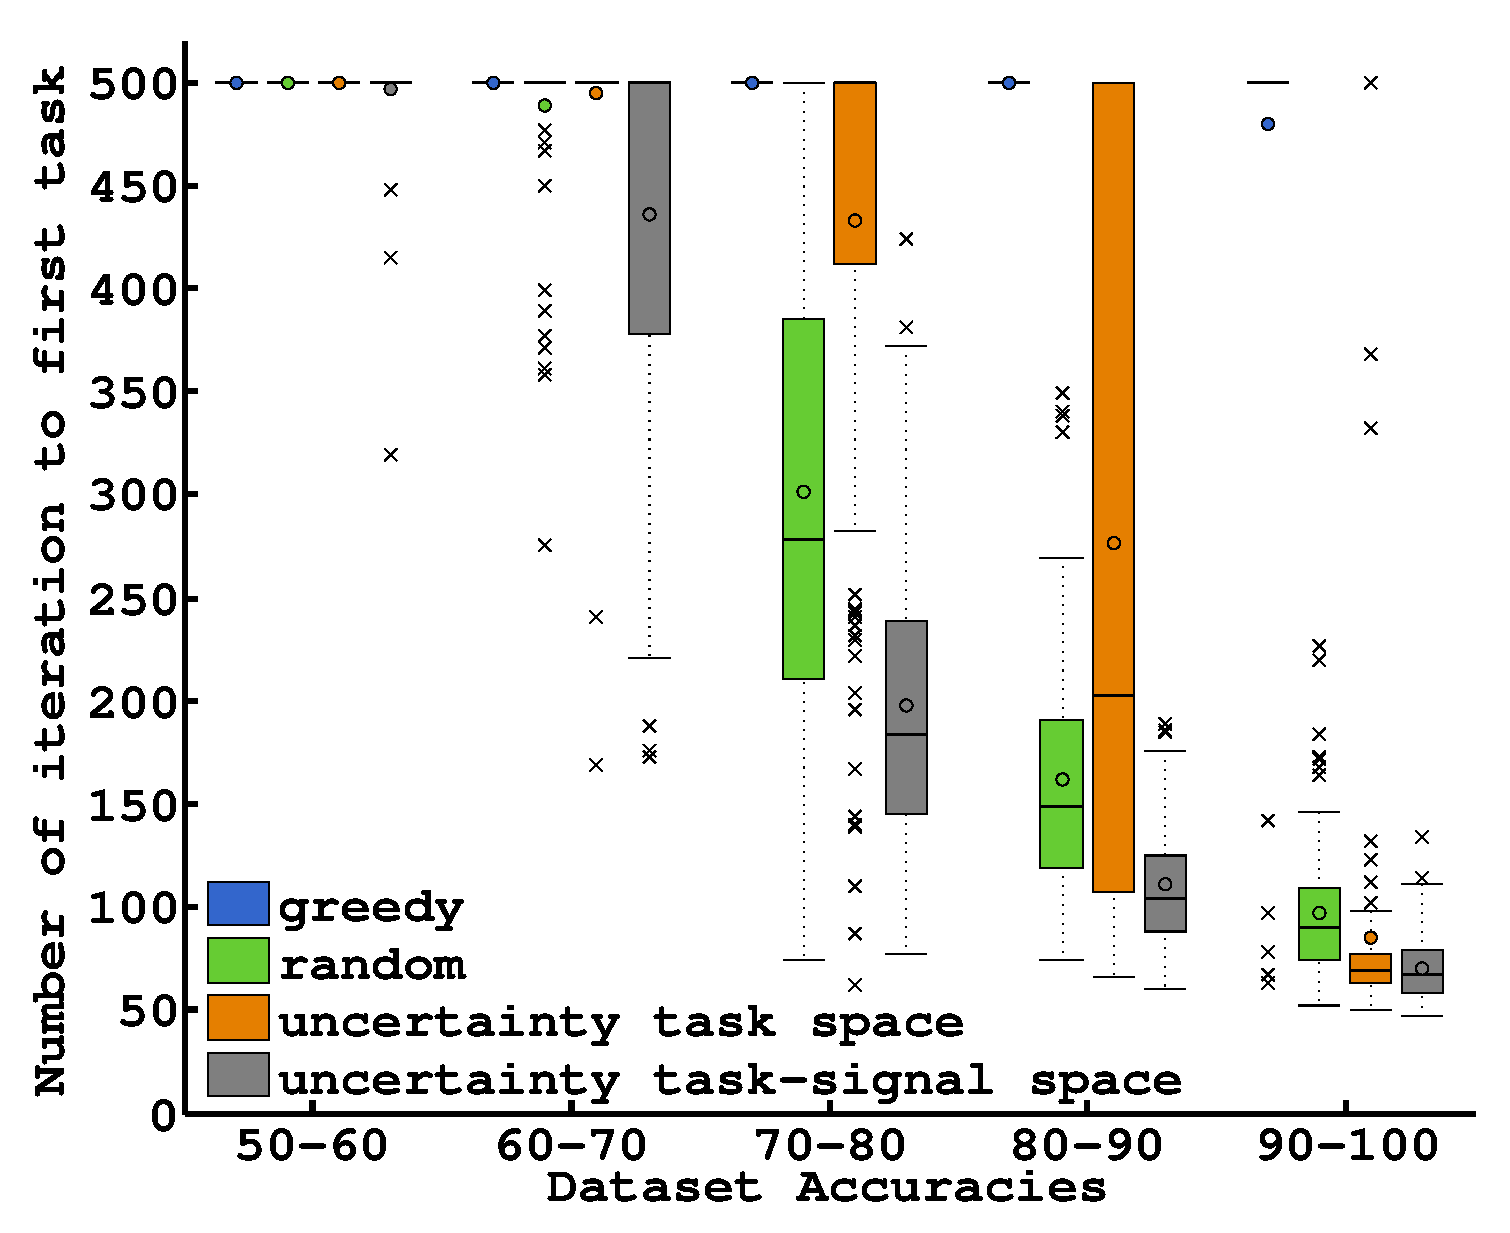
\includegraphics[width=\columnwidth]{img/plots_aaai/plot_artificial_planning.eps}
      \caption{Number of steps to complete first task, comparison of different exploration methods with 30 dimensional artificial data. When learning from scratch, planning upon uncertainty in both task and signal space performs better than relying only on task uncertainty. Greedy action selection rarely disambiguates between hypothesis.}
    \label{fig:planning}
\end{figure}

As depicted in Figure~\ref{fig:planningExplained}, the system needs to collect two types of information, some about the true underlying model (Fig.~\ref{fig:planningExplained}b) and some to differentiate between hypotheses (Fig.~\ref{fig:planningExplained}a). The properties of the grid world make the random strategy quite efficient at collecting those two types of information. The differences between planning methods should be more evident when navigating a complex maze since our method allows to plan in order to collect the type of information we need. Studying how different world properties affect the learning efficiency is part of our future work. Also, we note that all planning methods were switched to pure exploitation (greedy) once the confidence level was reached. Therefore the performance in Figure~\ref{fig:planning} compares the ability of the different methods to discriminate between different task hypotheses, not their ability to solve the task itself.

\paragraph{Dimensionality}

Figure~\ref{fig:firstArtificial} compares the number of steps (with maximum values of 500 steps) needed to identify the first task when learning from scratch with different dimensionality of datasets. The convergence speed is only slightly affected by the features dimensionality. On the other hand, the dataset quality (measured in terms of it associated ten-fold accuracy) is the main cause of performances decay. Furthermore, for those datasets with accuracies between $50\%$ and $60\%$, the system is not able to identify a task with confidence after 500 steps.

\begin{figure}[!ht]
  \centering
      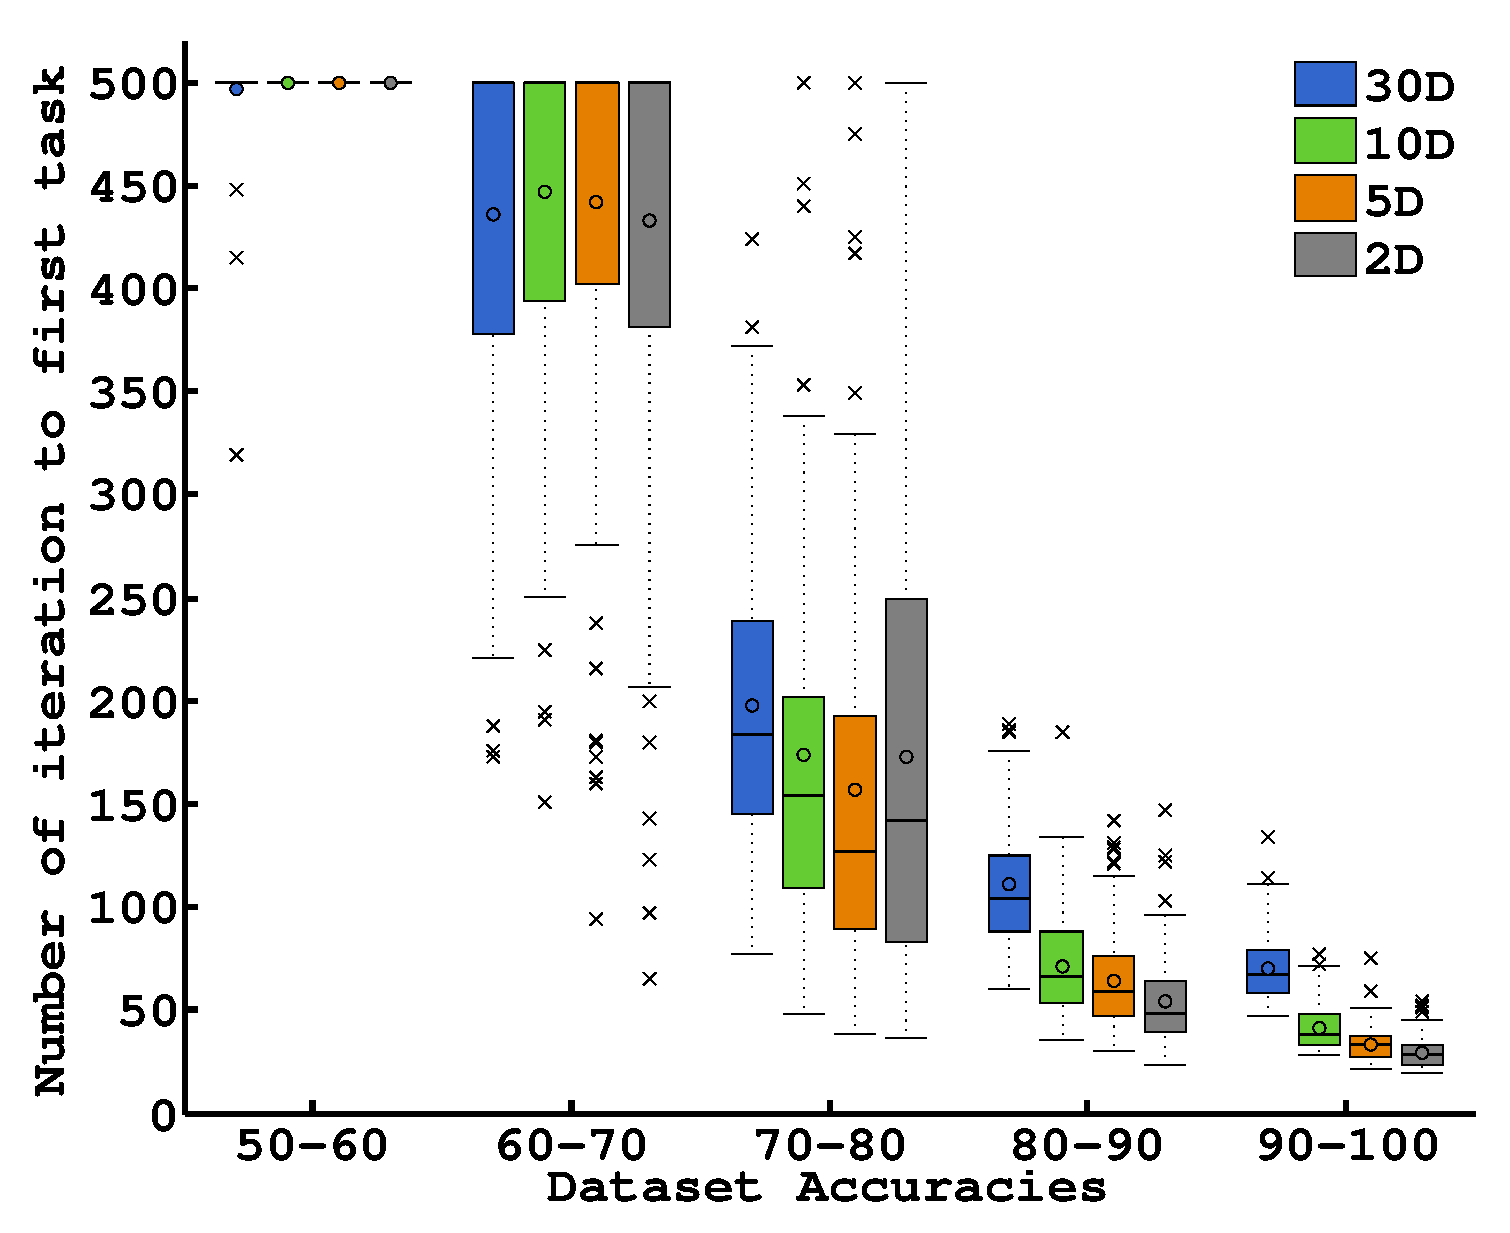
\includegraphics[width=\columnwidth]{img/plots_aaai/plot_artificial_firstconf.eps}
      \caption{Number of steps to complete first task using artificial data. Under 60 percent accuracy, the confidence threshold cannot be reached in 500 steps. The dataset qualities, more than their dimensionality, impact the learning time.}
      \label{fig:firstArtificial}
\end{figure} 

Once one task is completed, a new one is selected randomly. Figure~\ref{fig:nCorrectArtificial} compares the number of tasks that can be achieved in 500 steps. As expected, the lower the quality of the data, the less number of task can be completed. With dataset accuracies higher than $90\%$ we can achieve more than 30 tasks on average.

\begin{figure}[!ht]
    \centering
    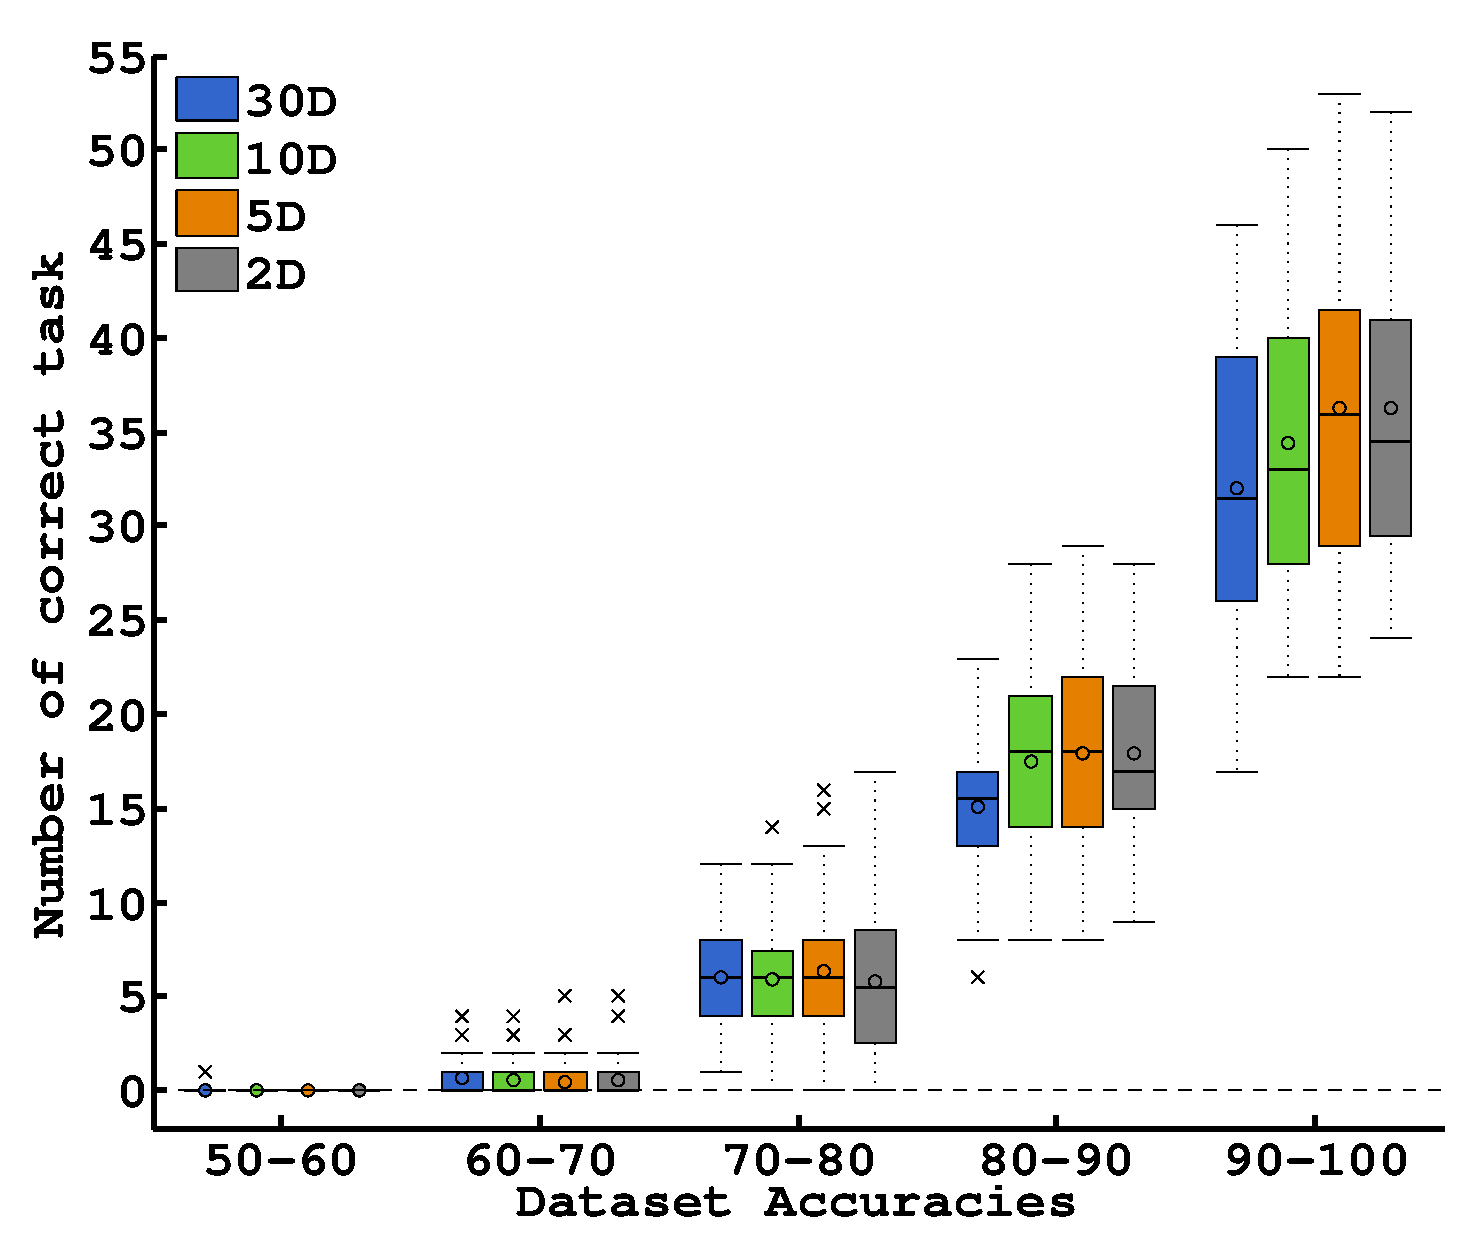
\includegraphics[width=\columnwidth]{img/plots_aaai/plot_artificial_nCorrect.eps}
    \caption{Number of tasks correctly achieved in 500 steps, artificial data. Quality of dataset impacts the number of task identified in 500 steps as more evidence should be collected to reach the confidence threshold.}
    \label{fig:nCorrectArtificial}
\end{figure} 

An important aspect of the proposed learning approach was that the first task learned was always the correct one. We reported only 9 erroneous estimations across all simulated experiments (5 in the 70-80 group and 4 in the 80-90 group).

\subsection{EEG datasets and comparison with calibration method}

\paragraph{Example}
Figure~\ref{fig:sequence} shows one particular run of 500 steps comparing our self-calibration method with a calibration procedure of 400 steps. The two independent runs use as real EEG dataset with $80\%$ ten-fold classification accuracy. As our algorithm is operational from the first step, it can estimate the real task when sufficient evidence has been collected. On the other hand, a calibration approach collects signal-label pairs for a fixed number of steps and use the resulting classifier without updating it. This provokes that, during the calibration phase, no tasks can be learned, substantially delaying the user's online operation.

\begin{figure}[!ht]
\centering
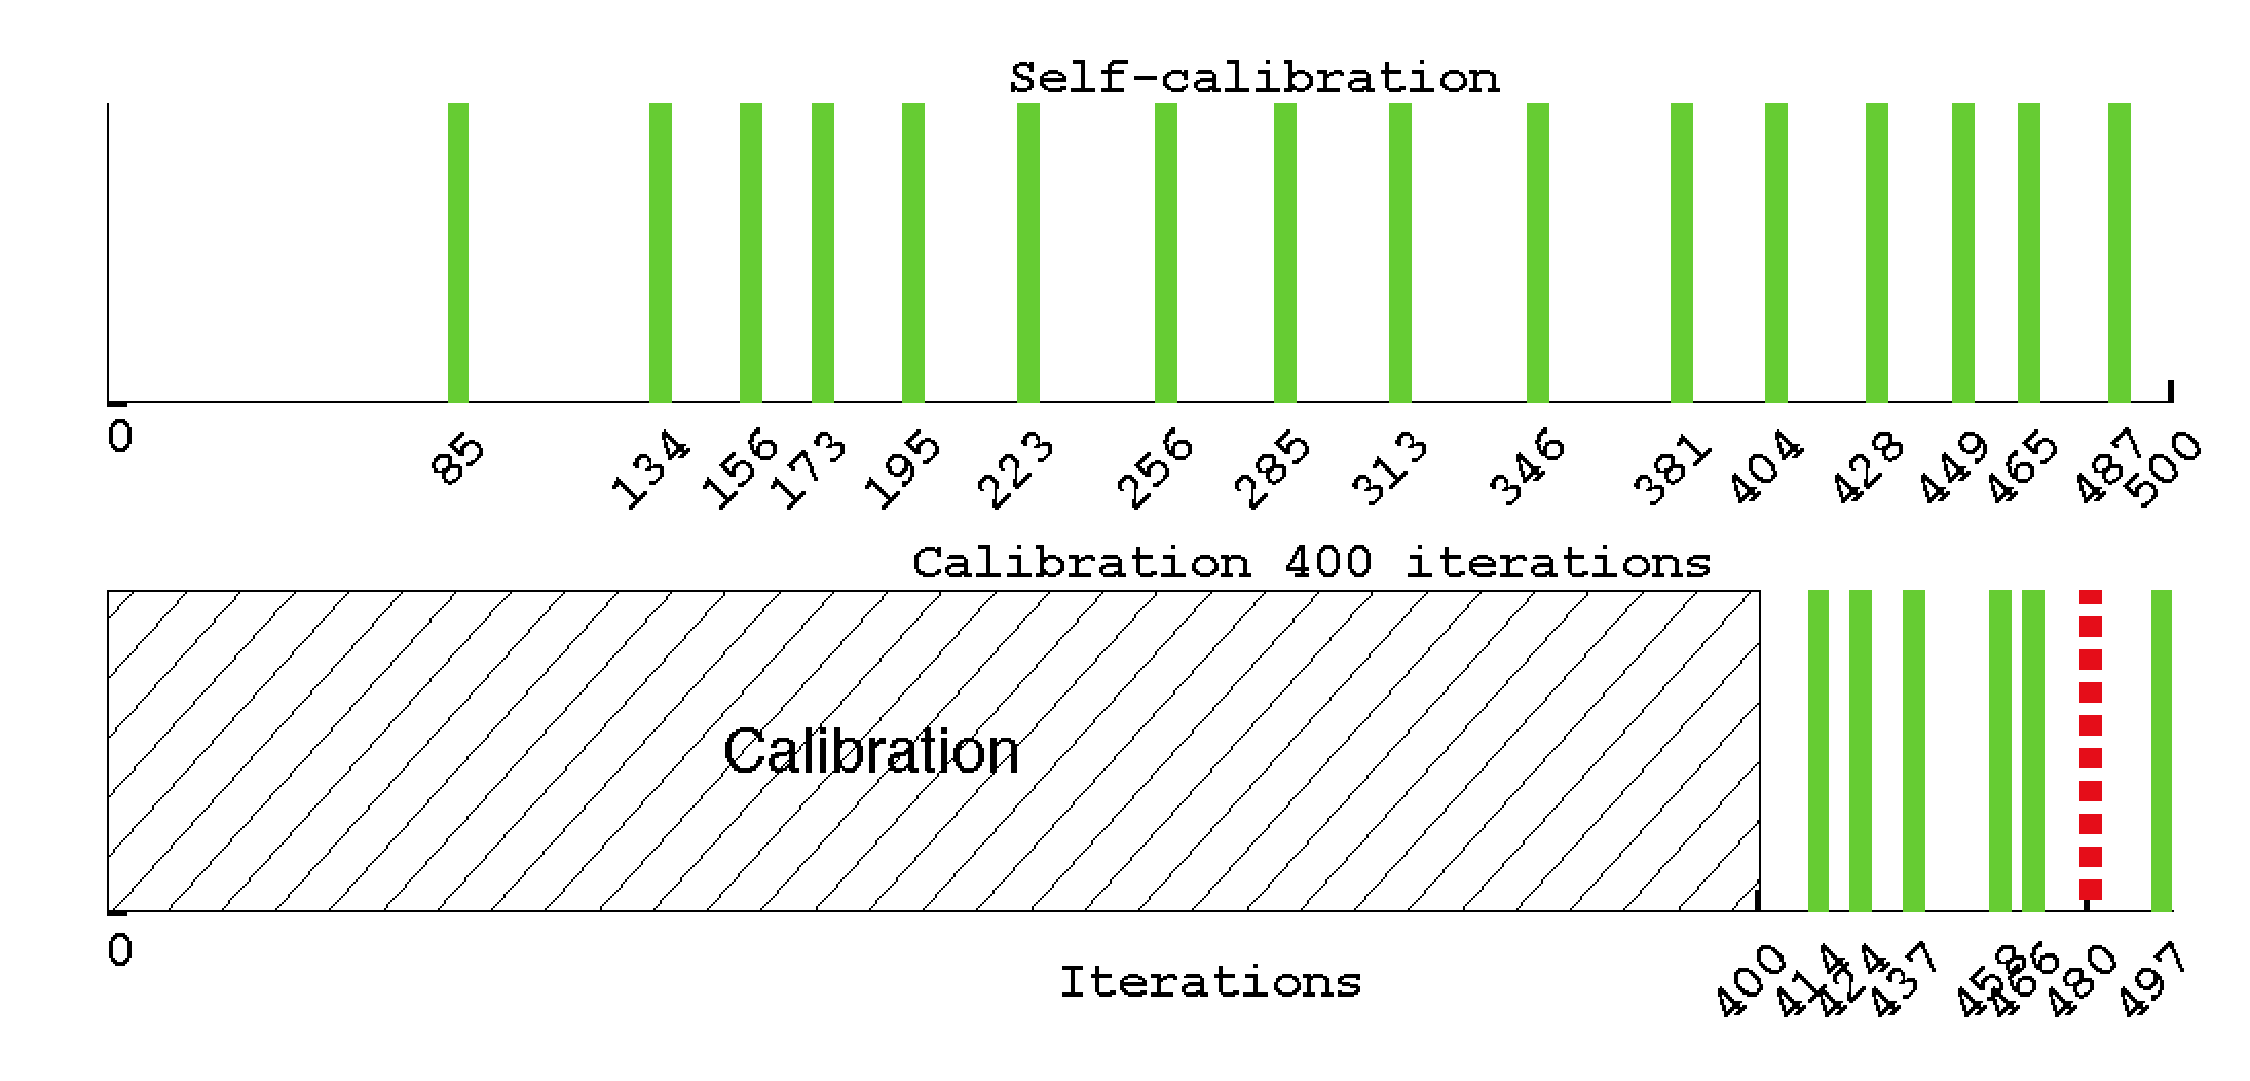
\includegraphics[width=\columnwidth]{img/plots_aaai/plot_the_aaai_sequence.eps}
\caption{Time-line of one run from EEG dataset of $80$ percent ten-fold classification accuracy, self-calibration (top) versus 400 steps calibration (bottom). Green (filled) and red (dashed) bars represents respectively correct and incorrect task achievement. The proposed self-calibration method allow to reach a first task faster than would take a calibration procedure.}
\label{fig:sequence}
\end{figure} 



Figure~\ref{fig:sequence_evolution} shows the evolution of classification rate between our self-calibration method with a calibration procedure of 400 steps. As our method assigns different labels to each new teaching signal, the resulting classifiers have different performances, which help identifying the correct task. Once a task is identified (e.g.\ step 85 and 134), the corresponding labels are taken as ground truth, and all classifiers will have the same accuracies. As the agent starts exploring again to estimate the new tasks, all the classifiers except the true one will start to have worse accuracies again.

\begin{figure}[!ht]
\centering
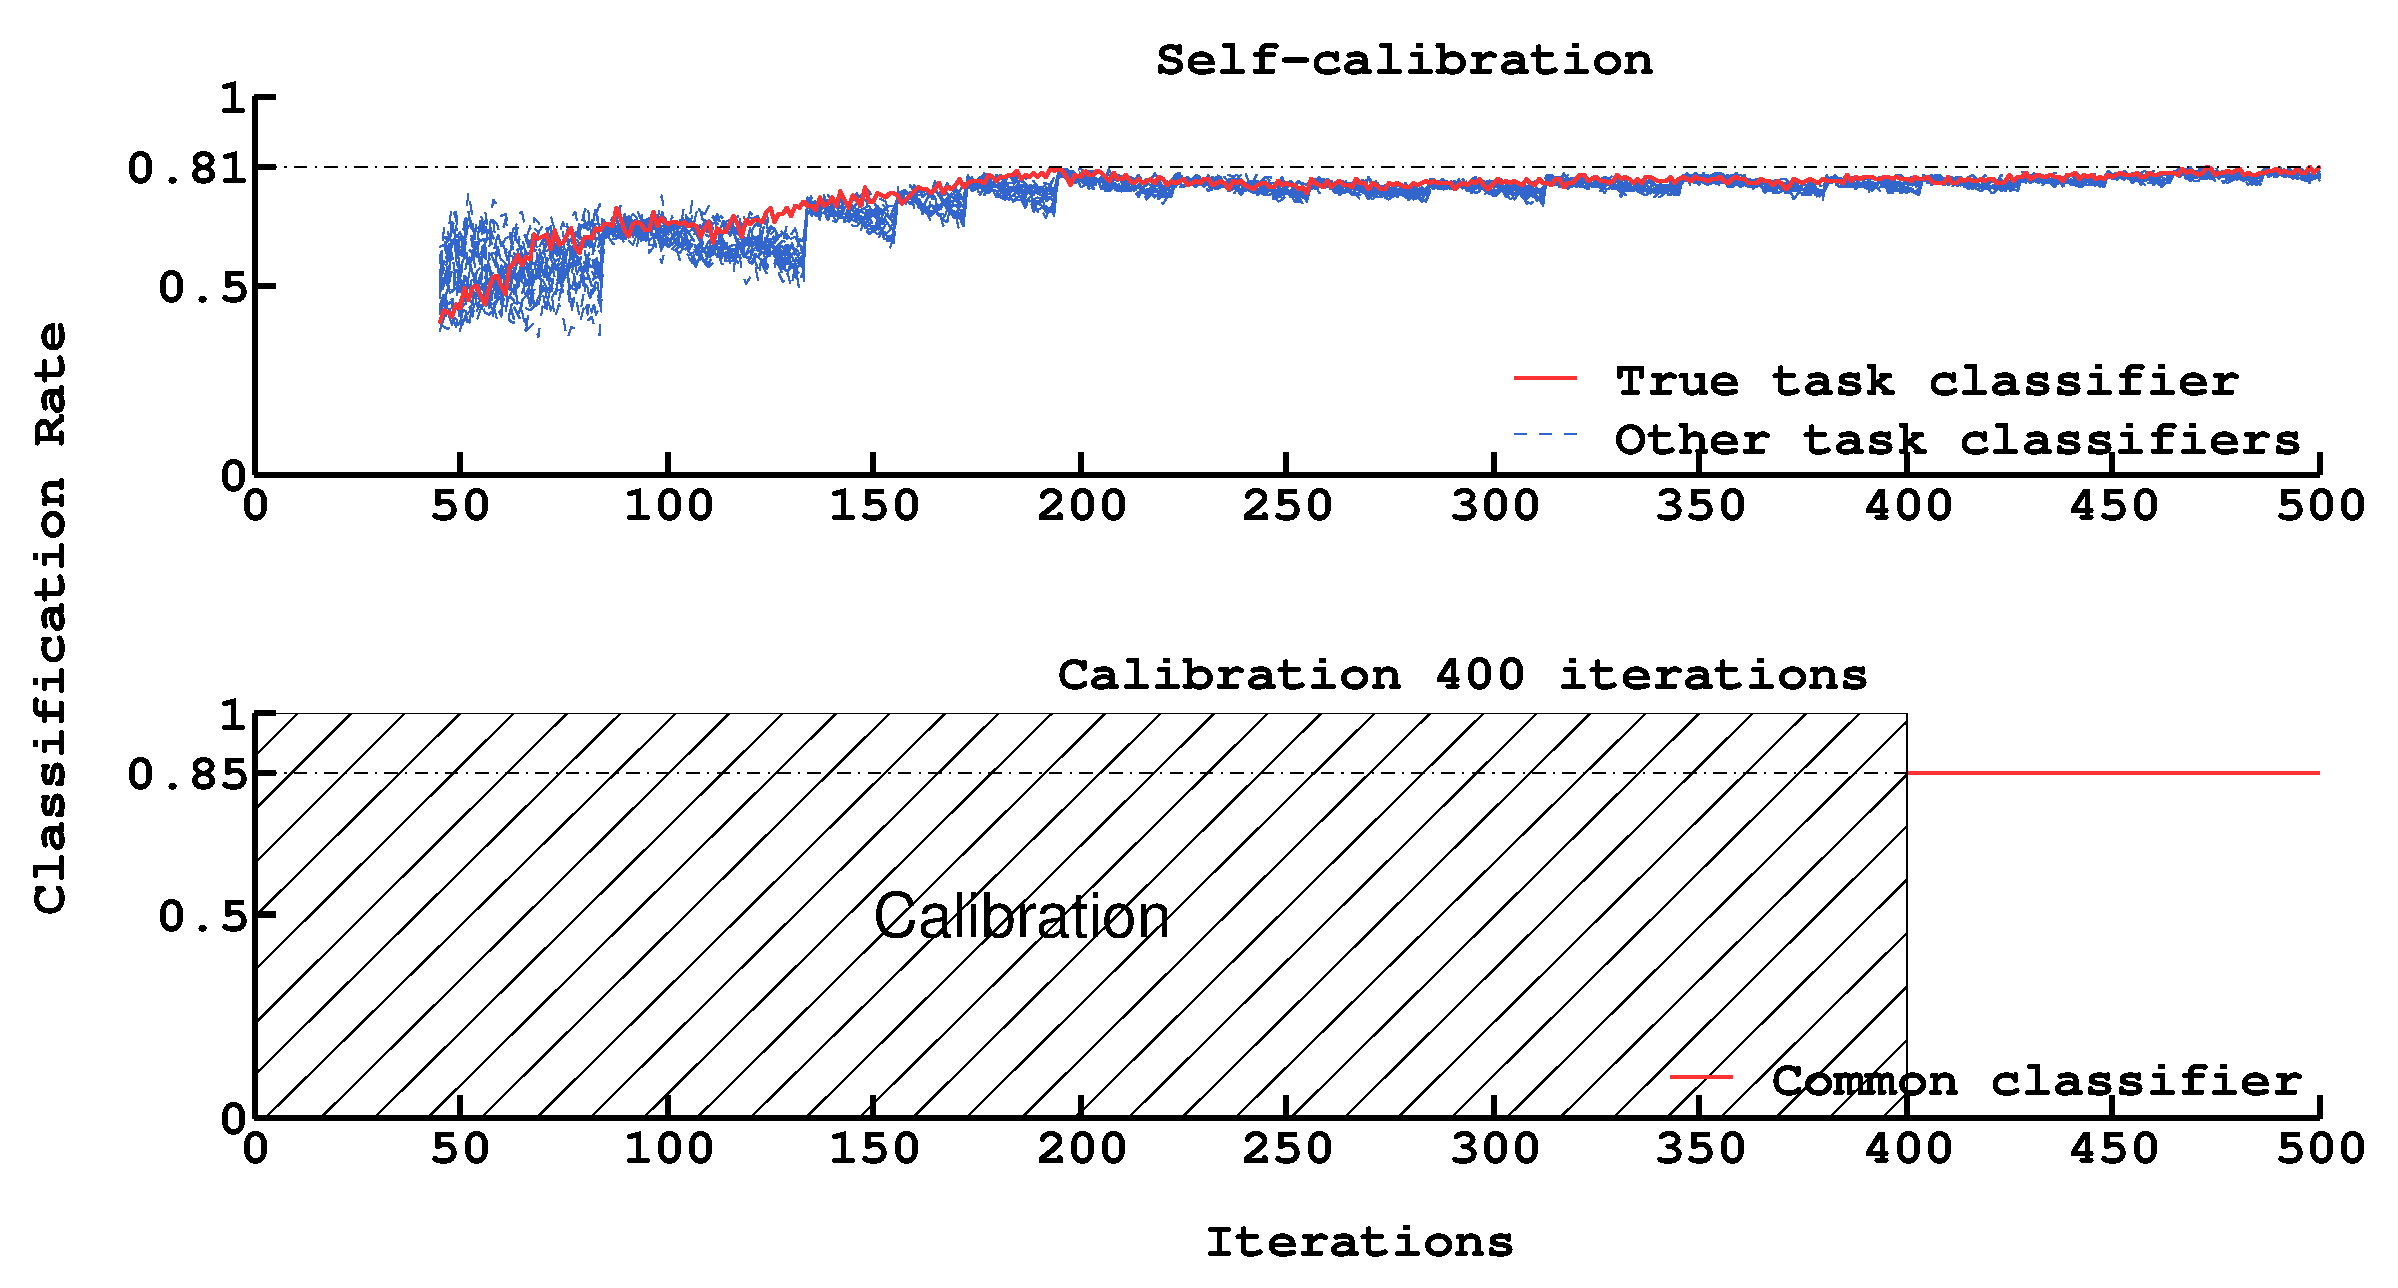
\includegraphics[width=\columnwidth]{img/plots_aaai/plot_evo_classification_rate.eps}
\caption{Evolution of classification rate of one run from EEG data, self-calibration (top) versus 400 steps calibration (bottom). On top, the red line represents the classifier corresponding to the successive tasks taught by the user, the dashed blue lines represent all others tasks. Our method updates classifiers every steps.}
\label{fig:sequence_evolution}
\end{figure} 

\paragraph{Time to first task}

Figure~\ref{fig:firstEEG} shows the results per group of dataset. Our algorithm allows to complete the first task without errors and in a fair amount of iteration.  For our method, the learning time is strongly correlated with the dataset quality. However calibration methods, which do not update their classifier once calibrated, identify more tasks incorrectly.

\begin{figure}[!ht]
\centering
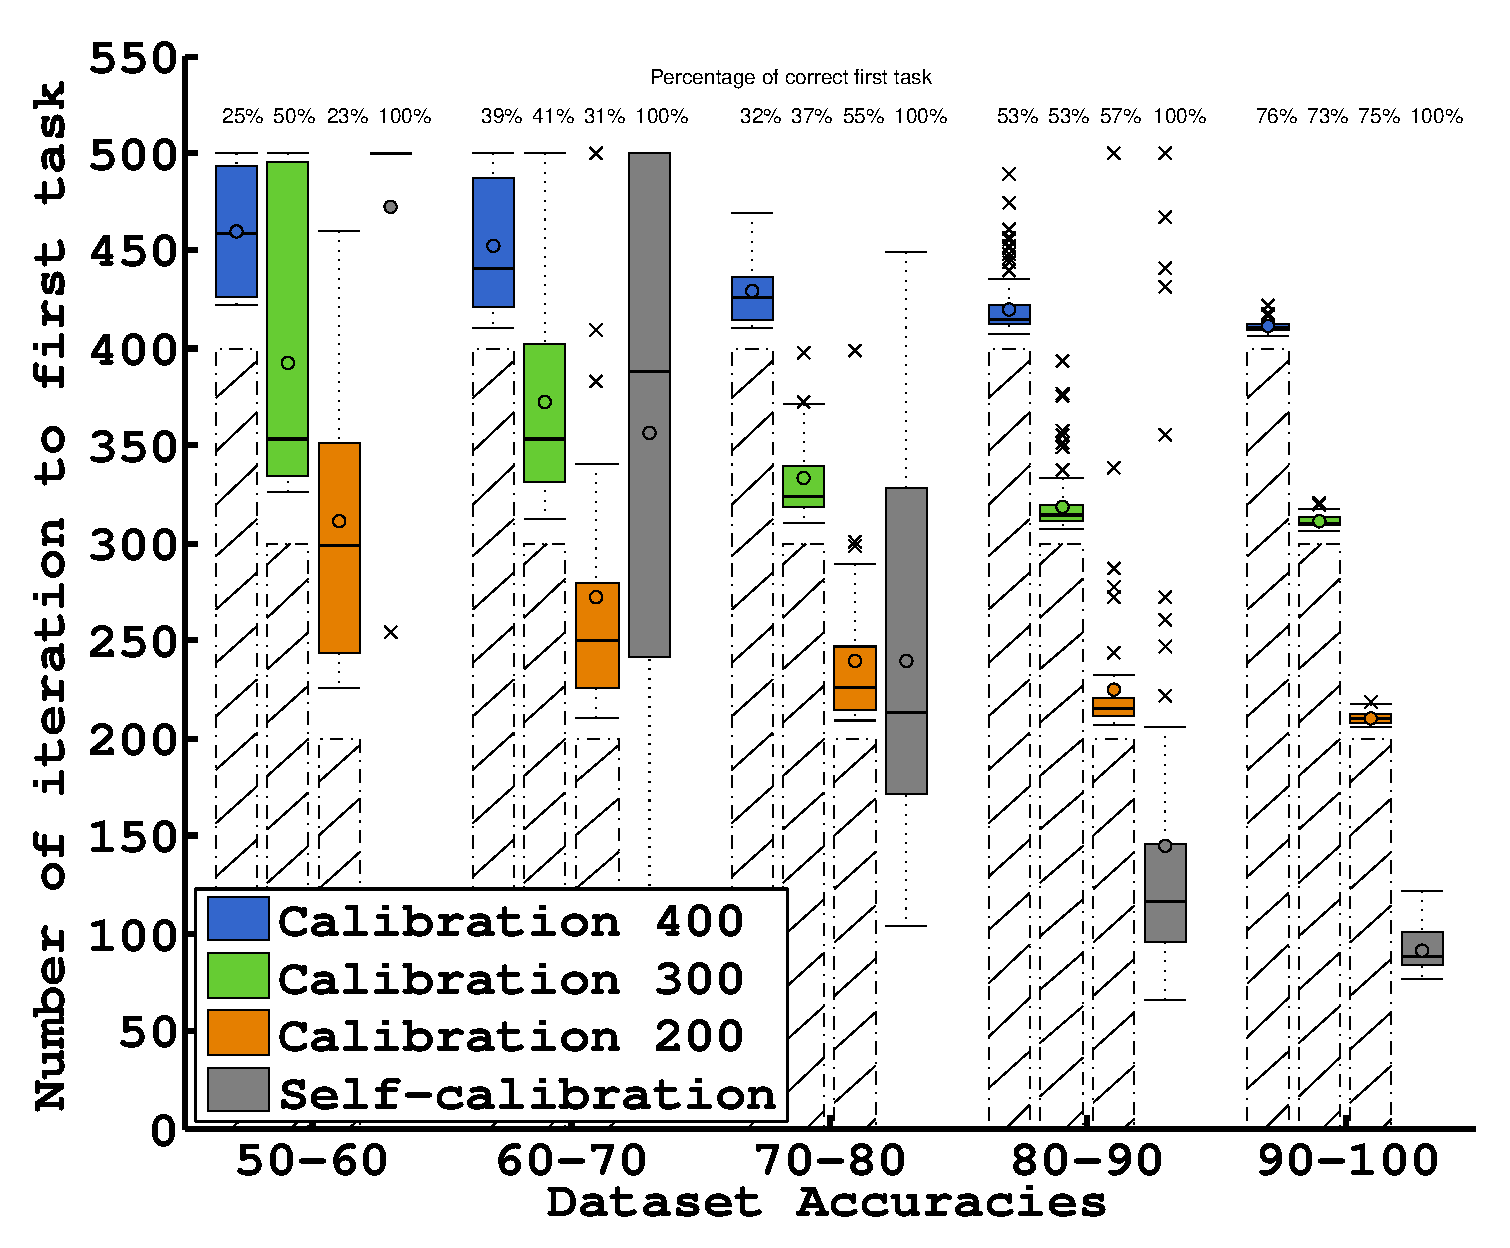
\includegraphics[width=\columnwidth]{img/plots_aaai/plot_EEG_calib_firstconf.eps}
\caption{Number of steps to complete first task with EEG data. The method scale well to EEG data. Contrary to the standard calibration approaches, we do not make mistakes with low quality datasets.}
\label{fig:firstEEG}
\end{figure} 

%We can identify two main differences between our method and the usual calibration procedure for this kind of BCI experiments:
%\begin{enumerate}
%\item \textbf{Positive/Negative percent ratio of training examples}. Following the literature \cite{chavarriaga2010learning, iturrate2013task} we used a 80/20 percent ratio. Table \ref{tab:correctLabelRatio} shows the positive/negative ratio obtained following our planning method. The ratio we obtain is more balanced, resulting in classifiers with better properties. However a 50/50 percent ratio may lead to practical problems during online real world experiments and should be studied in more details, see open questions in section \ref{sec:conclusion}.
%\item \textbf{Online update of multiple classifiers.} Our method integrates new data at every step whose label can differ between task hypothesis. For incorrect task hypothesis, the associated label can be incorrect and decrease the performance of the associated classifier, see figure \ref{fig:planningExplained}c. This dynamic can be observed in figure \ref{fig:sequence_evolution} where classifiers associated to incorrect tasks (in blue) have lower estimated accuracies than the correct one (in red). As a result our algorithm makes different predictions and updates for each hypothesis.
%\end{enumerate}

%\begin{table}
%\begin{tabular}{c c c}
%Dataset Accuracies & Self-calibration & Calibration \\ \hline
%50-60 & 0.48 (0.02) & 0.8 (0) \\
%60-70 & 0.50 (0.03) & 0.8 (0) \\
%70-80 & 0.53 (0.03) & 0.8 (0) \\
%80-90 & 0.57 (0.03) & 0.8 (0) \\
%90-100 & 0.59 (0.01) & 0.8 (0) \\
%\end{tabular}
%\caption{Mean ratio of positive examples in training dataset (standard deviation shown in parenthesis). Calibration procedure for ErP EEG signal usual account for a 80 percent ratio of positive examples. However when following our method we collect as many positive than negative examples, see discussion in section \ref{sec:conclusion}.}
%\label{tab:correctLabelRatio}
%\end{table}

%\begin{figure}[!ht]
%\centering
%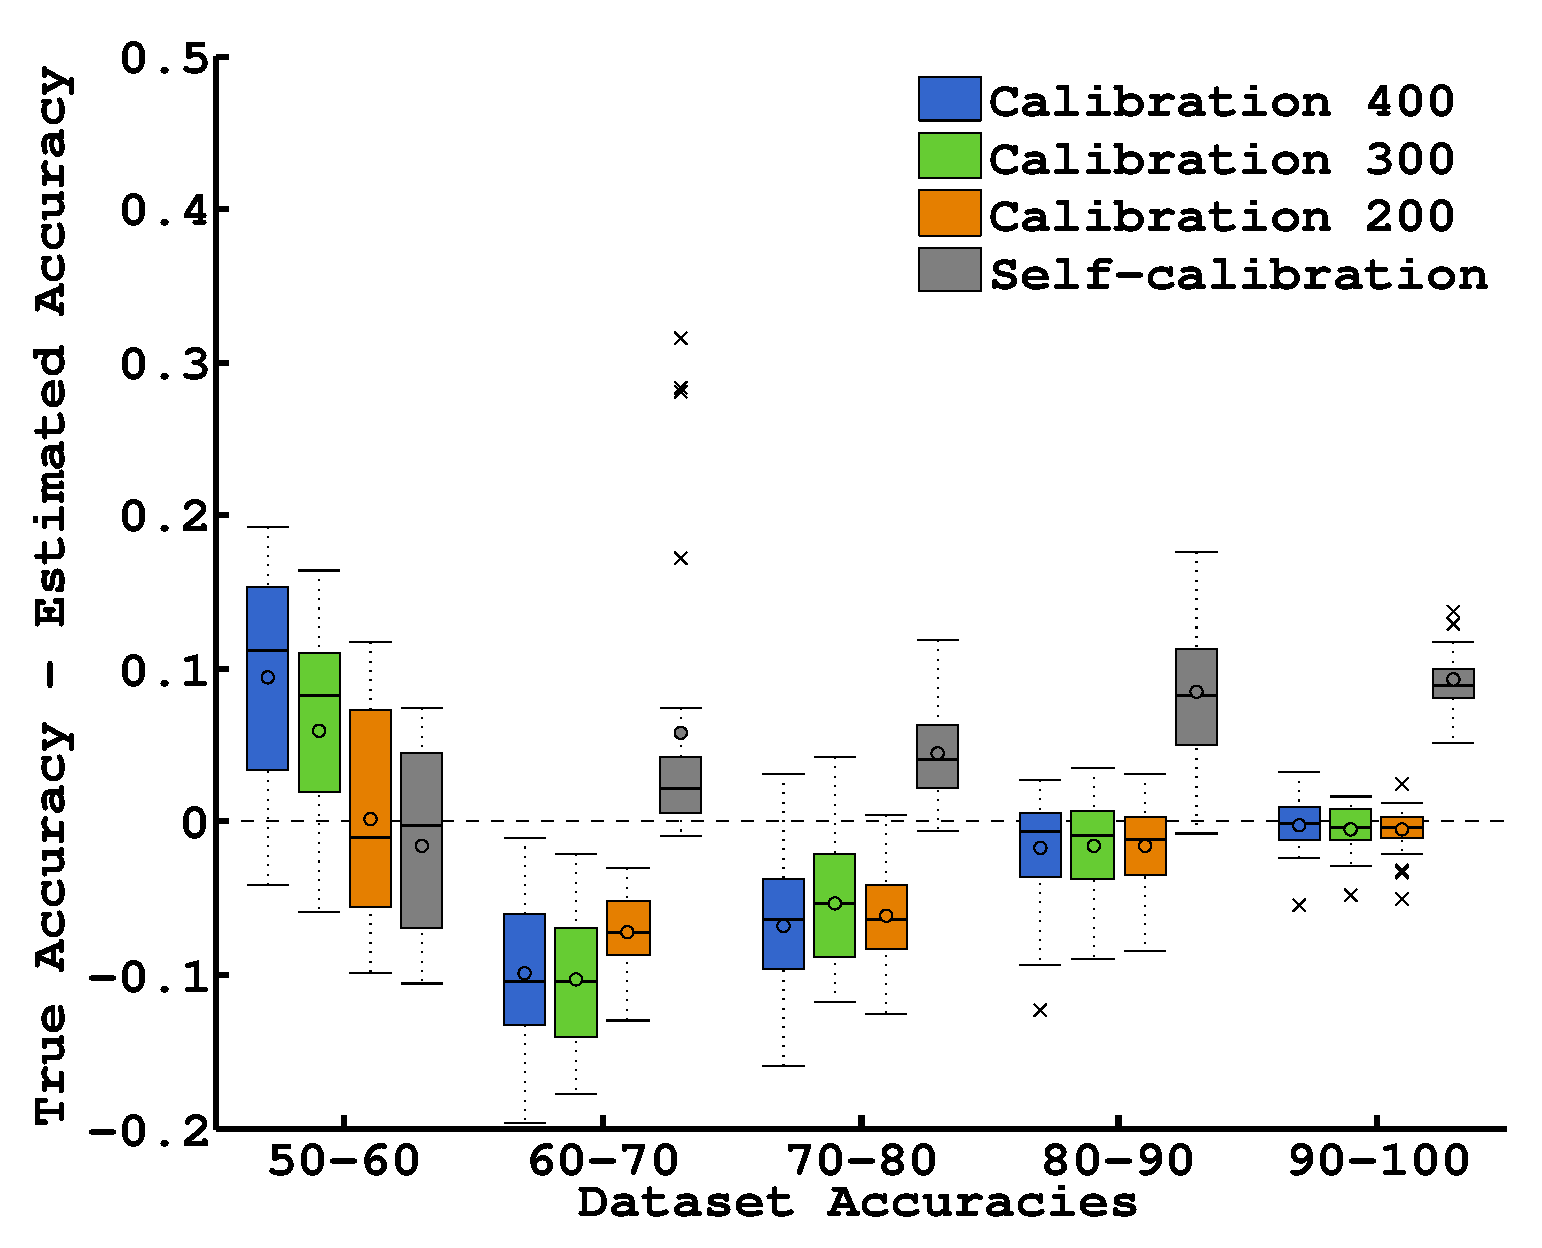
\includegraphics[width=\columnwidth]{img/plots_aaai/plot_explaination_for_calib_failure.eps}
%\caption{Difference between true accuracy and estimated accuracy. True accuracy is the performance of the classifier on the unused data. Estimated accuracy is the 10 fold cross validation performance of the classifier on collected data. A negative(positive) value indicates the classifier is over(under)-estimating its performance. Calibration methods tend to produce over-confident classifiers, certainly due to the biased positive to negative training example ratio, see table \ref{tab:correctLabelRatio}.}
%\label{fig:calibFail}
%\end{figure}

\paragraph{Cumulative performances}

Figure~\ref{fig:nCorrectEEG} compares the number of tasks that can be achieved in 500 steps. With 90\% and more dataset quality we can achieve about 20 tasks on average. The results are consistent with artificial dataset analysis.

\begin{figure}[!ht]
\centering
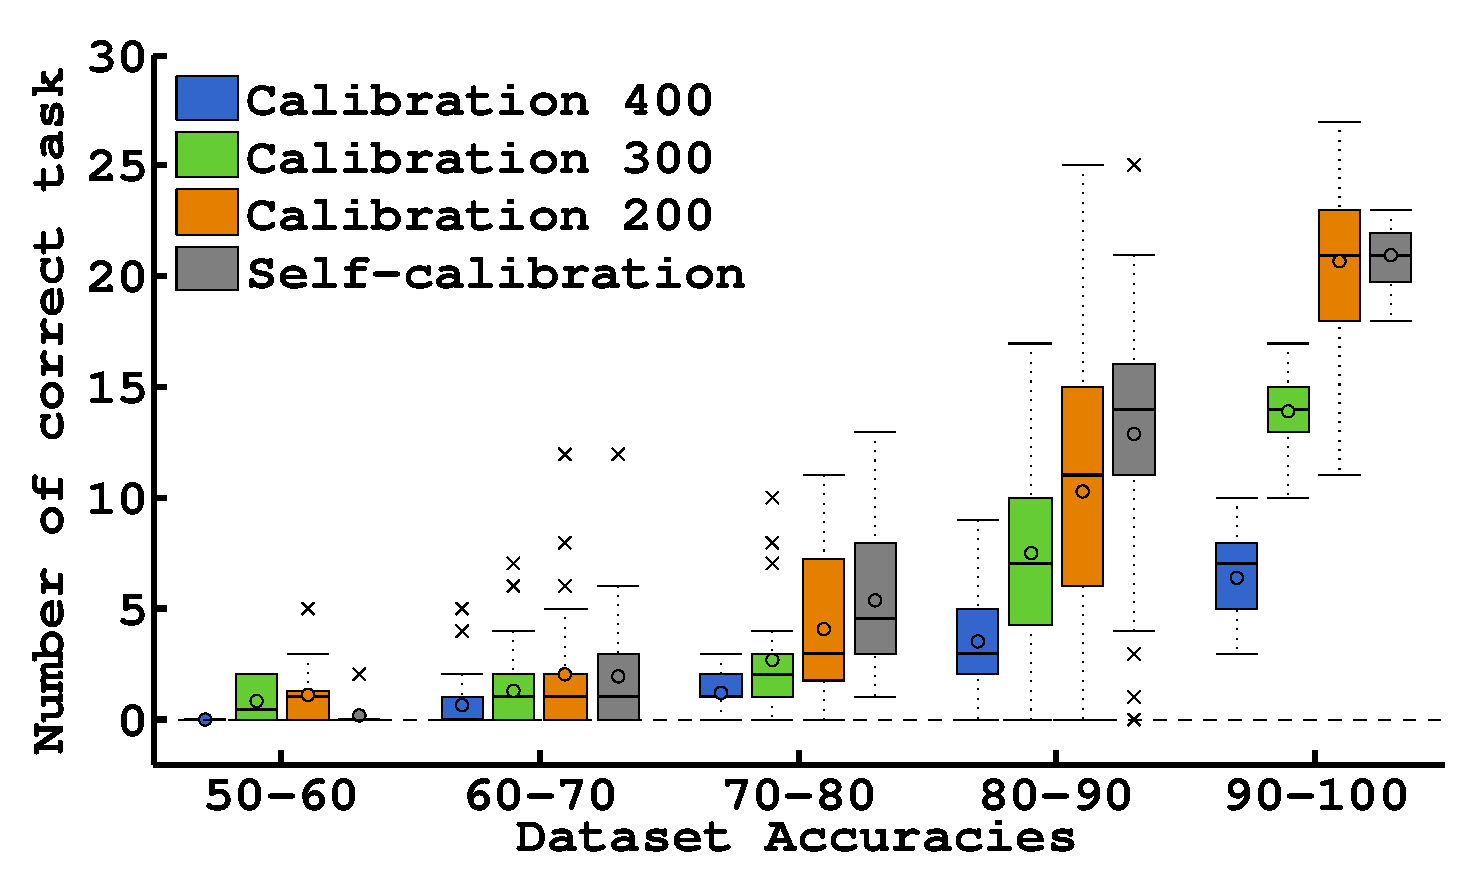
\includegraphics[width=\columnwidth]{img/plots_aaai/plot_EEG_calib_nCorrect.eps}
\caption{Number of task correctly achieved in 500 steps with EEG data. Calibration methods can not complete a significant number of task as most of the time is spent on calibration.}
\label{fig:nCorrectEEG}
\end{figure} 

The calibration methods can not complete many task as a significant amount of iteration was used for calibrating the system. A calibration of 200 steps makes as many good estimation than our method, but it also makes many wrong estimation, see Figure~\ref{fig:nWrongEEG}. For calibration methods, the less time spent on calibration, the poorer the classifier which implies more mistakes.

\begin{figure}[!ht]
\centering
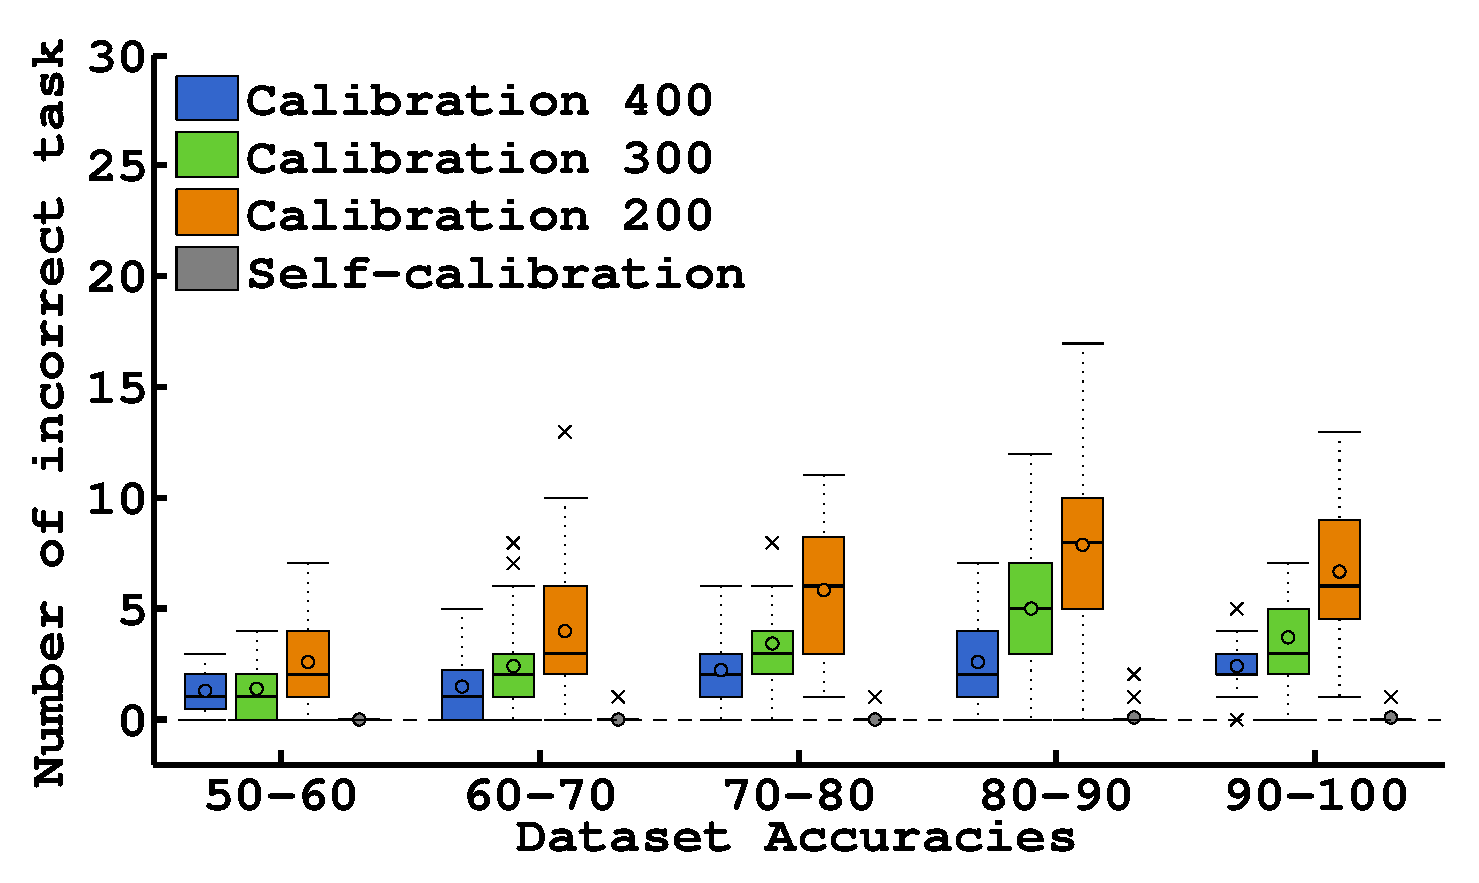
\includegraphics[width=\columnwidth]{img/plots_aaai/plot_EEG_calib_nWrong.eps}
\caption{Number of task incorrectly achieved in 500 steps with EEG data. Calibration methods, which do not update their models once calibrated, make more errors.}
\label{fig:nWrongEEG}
\end{figure}

%\paragraph{Last 100 iterations performances}
%
%Figure~\ref{fig:nCorrectEEG_last100} compares the number of task that can be achieved during the last 100 steps with EEG data. With 80-90\% dataset quality, all methods achieve an average success rate of one task every 20 steps. However calibration methods, which do not update their models once calibrated, make more mistakes (see figure \ref{fig:nWrongEEG_last100}).
%
%\begin{figure}[!ht]
%\centering
%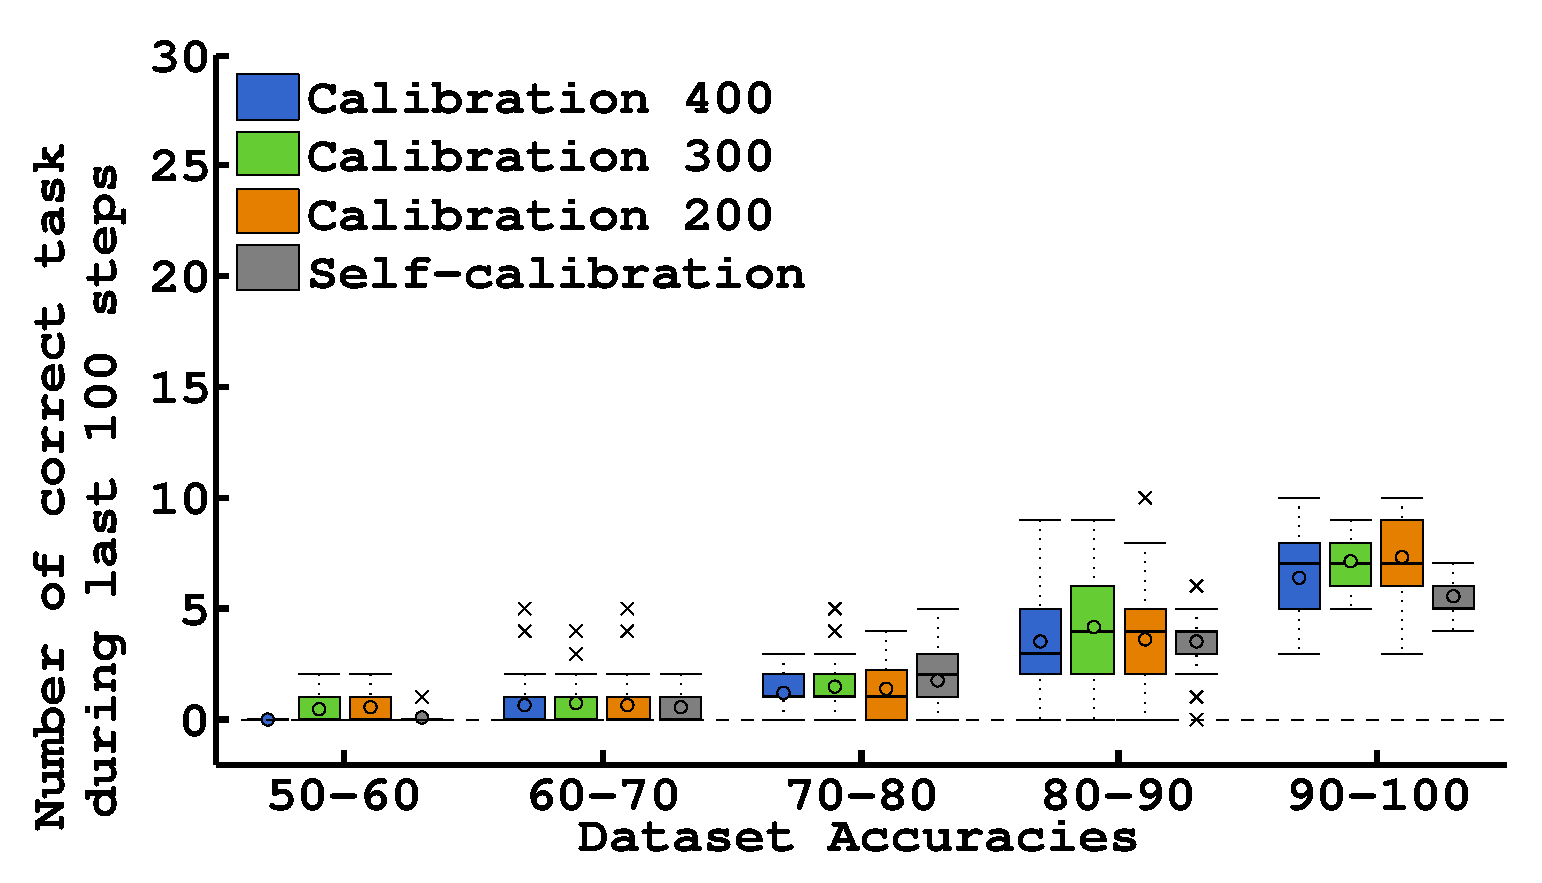
\includegraphics[width=\columnwidth]{img/plots_aaai/plot_EEG_calib_nCorrect_last100.eps}
%\caption{Number of task correctly achieved during the last 100 steps with EEG data. All methods have equivalent successful reaching rate.}
%\label{fig:nCorrectEEG_last100}
%\end{figure} 
%
%\begin{figure}[!ht]
%\centering
%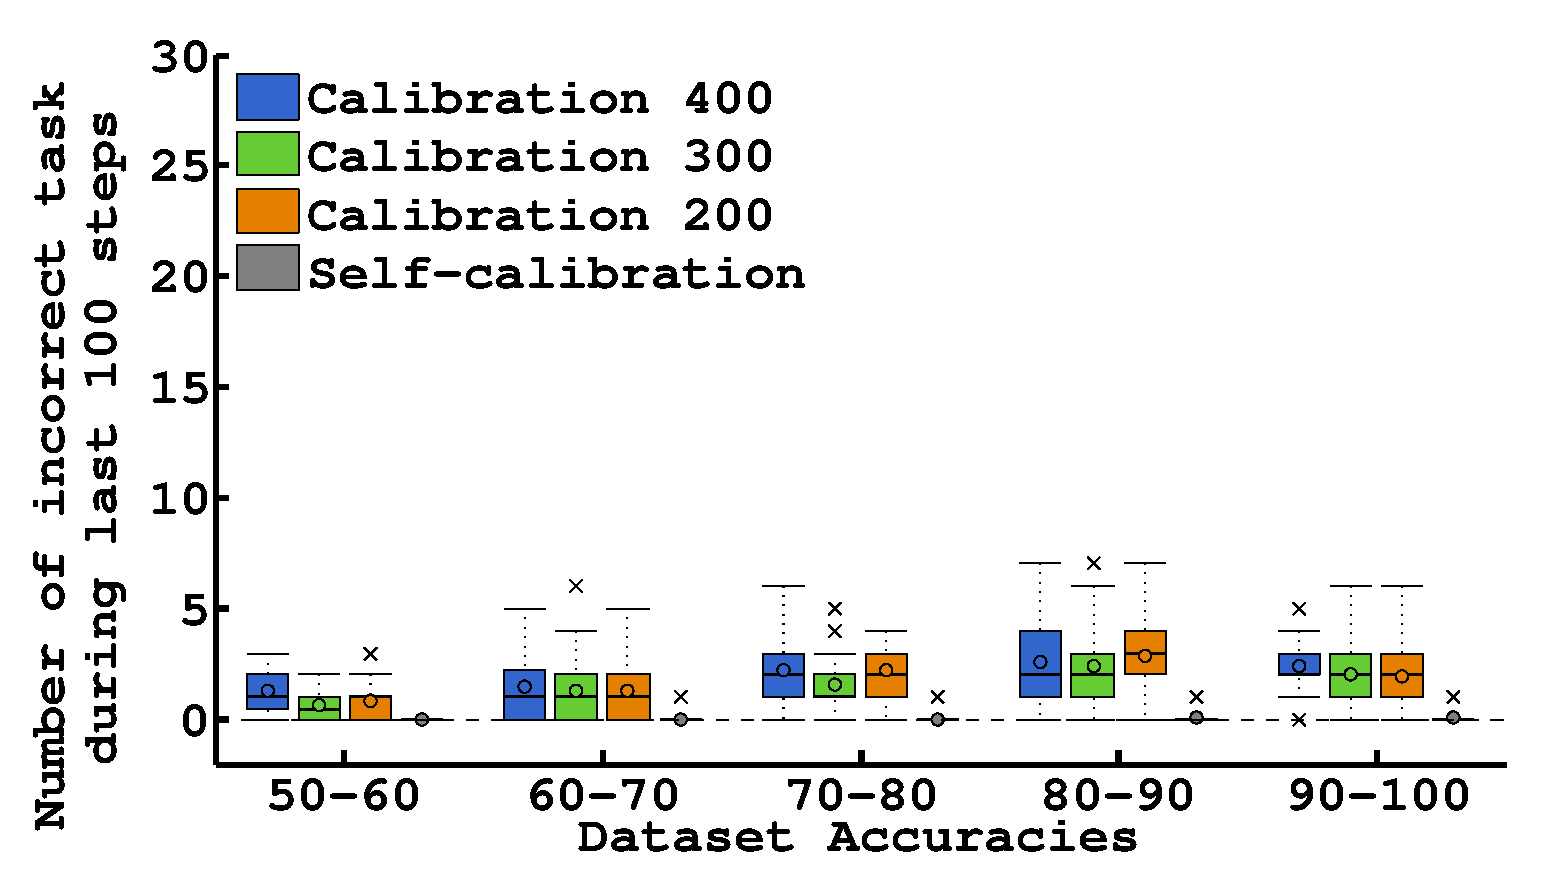
\includegraphics[width=\columnwidth]{img/plots_aaai/plot_EEG_calib_nWrong_last100.eps}
%\caption{Number of task incorrectly achieved during the last 100 steps with EEG data. Calibration methods, which do not update their models once calibrated, make more errors.}
%\label{fig:nWrongEEG_last100}
%\end{figure} 

 % shows the number of tasks identified with respect to the accuracy of the dataset, and the number of tasks incorrectly identified. Notice how the number of identified task is correlated to the quality of the dataset. Importantly, we were able to identify 15 to 20 tasks in 500 steps on good quality dataset without the need for a calibration procedure.


% \begin{figure*}[t]
% \centering
% \begin{minipage}[t]{.65\columnwidth}
% 	\centering
%    		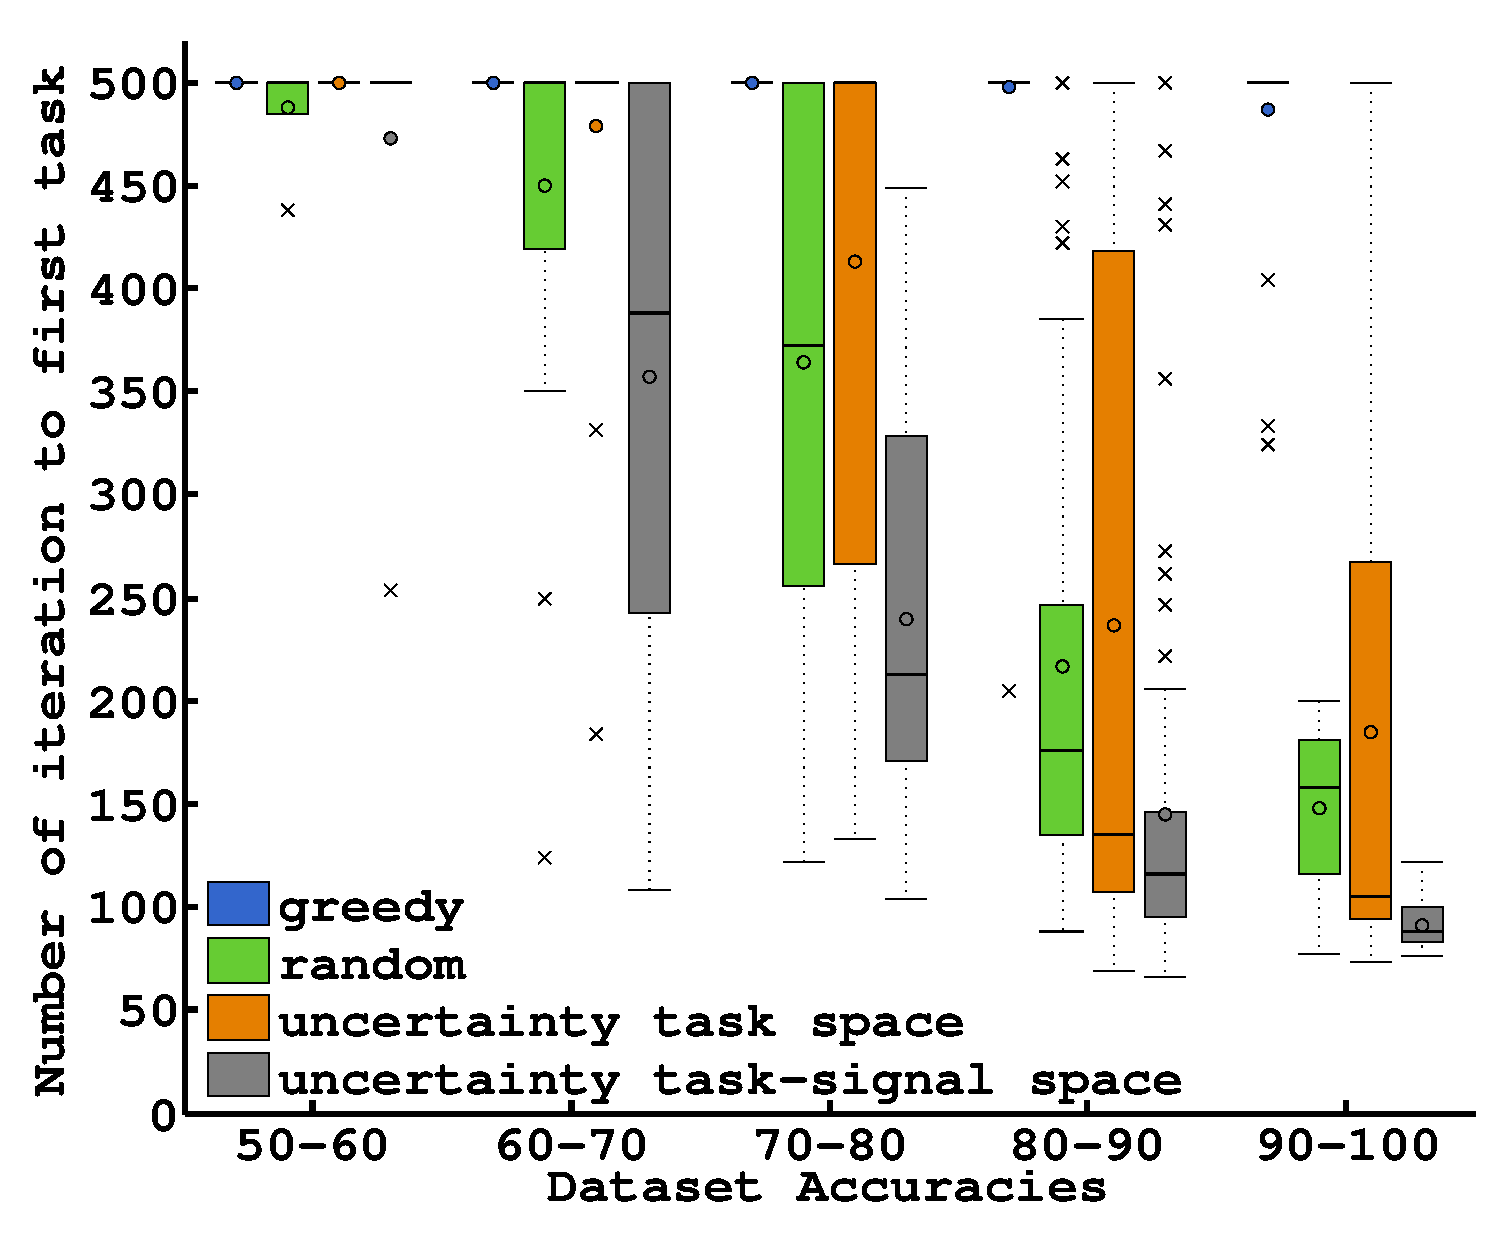
\includegraphics[width=\columnwidth]{img/plots_aaai/plot_EEG_planning.eps}
%    		\caption{\todo{this is the plot for EEG data, xp are running for artificial data}}
% 		\label{fig:planning}
% \end{minipage}
% \begin{minipage}[t]{.65\columnwidth}
% 	\centering
%    		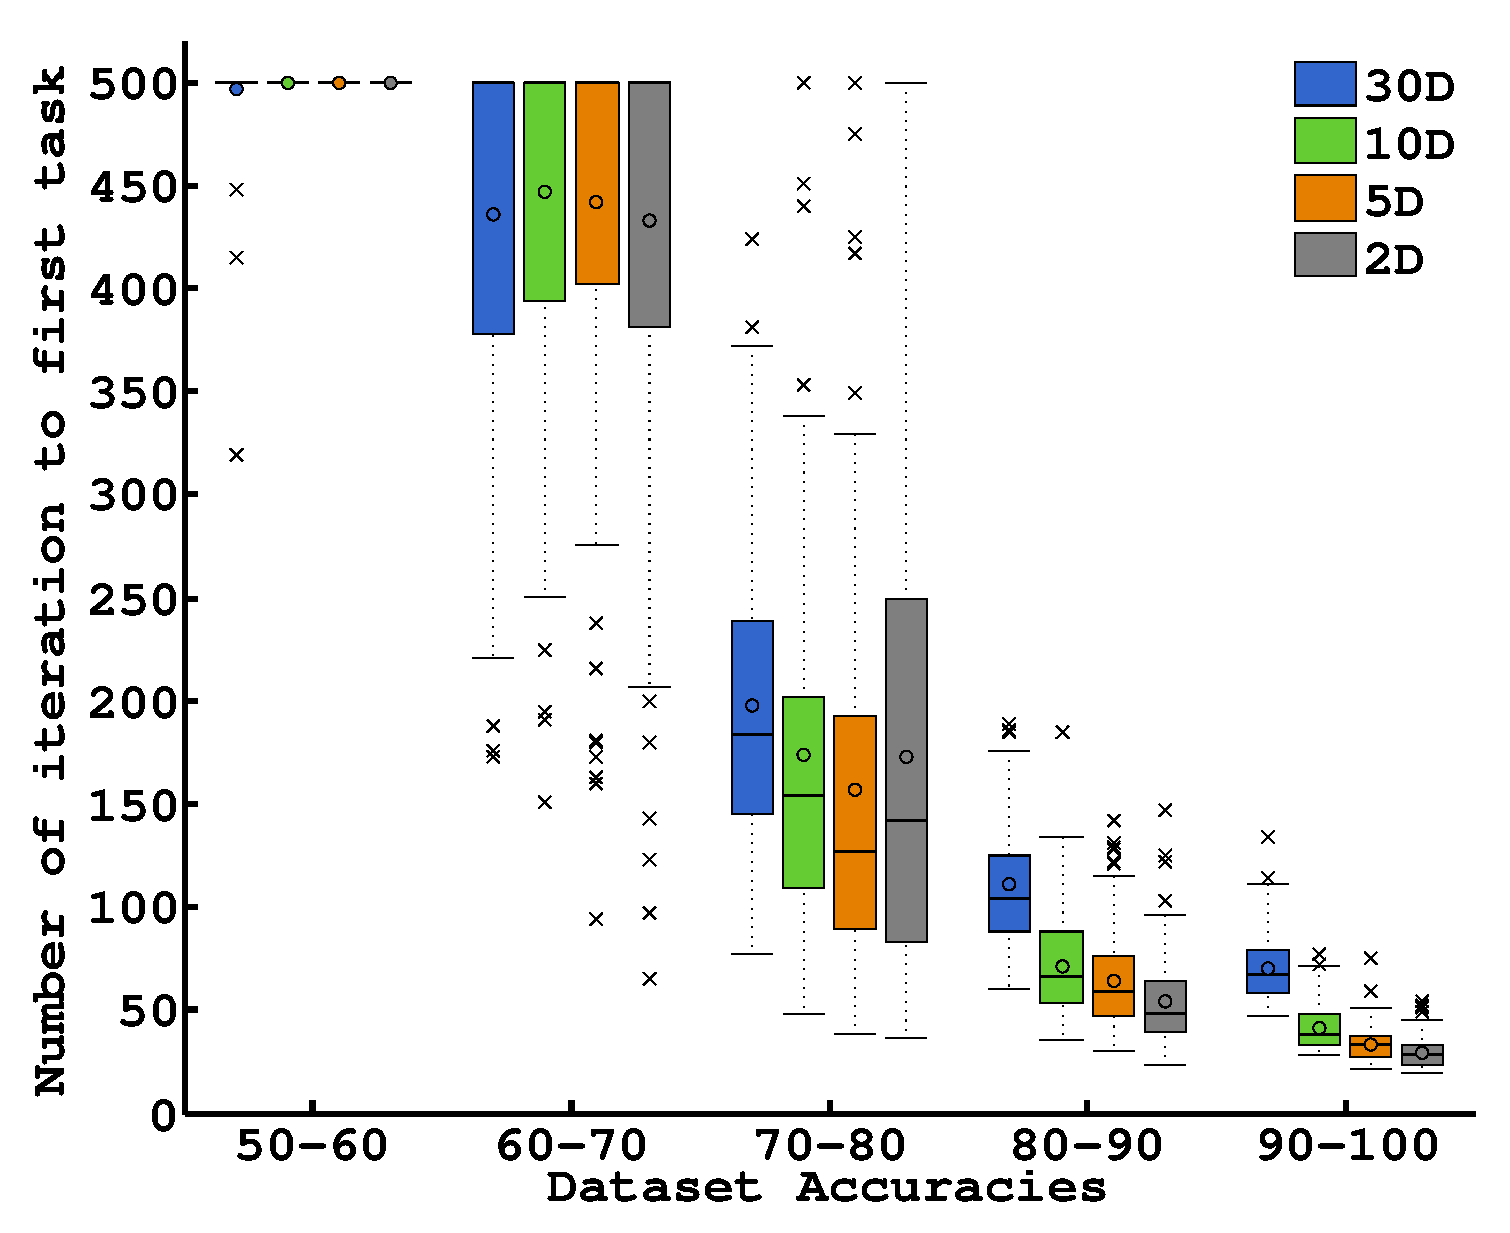
\includegraphics[width=\columnwidth]{img/plots_aaai/plot_artificial_firstconf.eps}
%    		\caption{Under 70 percent accuracy, the confidence threshold cannot be reached in 500 steps. The dataset qualities, more than their dimensionality, impact the learning time.}
%    		\label{fig:firstArtificial}
% \end{minipage}	
% \begin{minipage}[t]{.65\columnwidth}
% 	\centering
%    			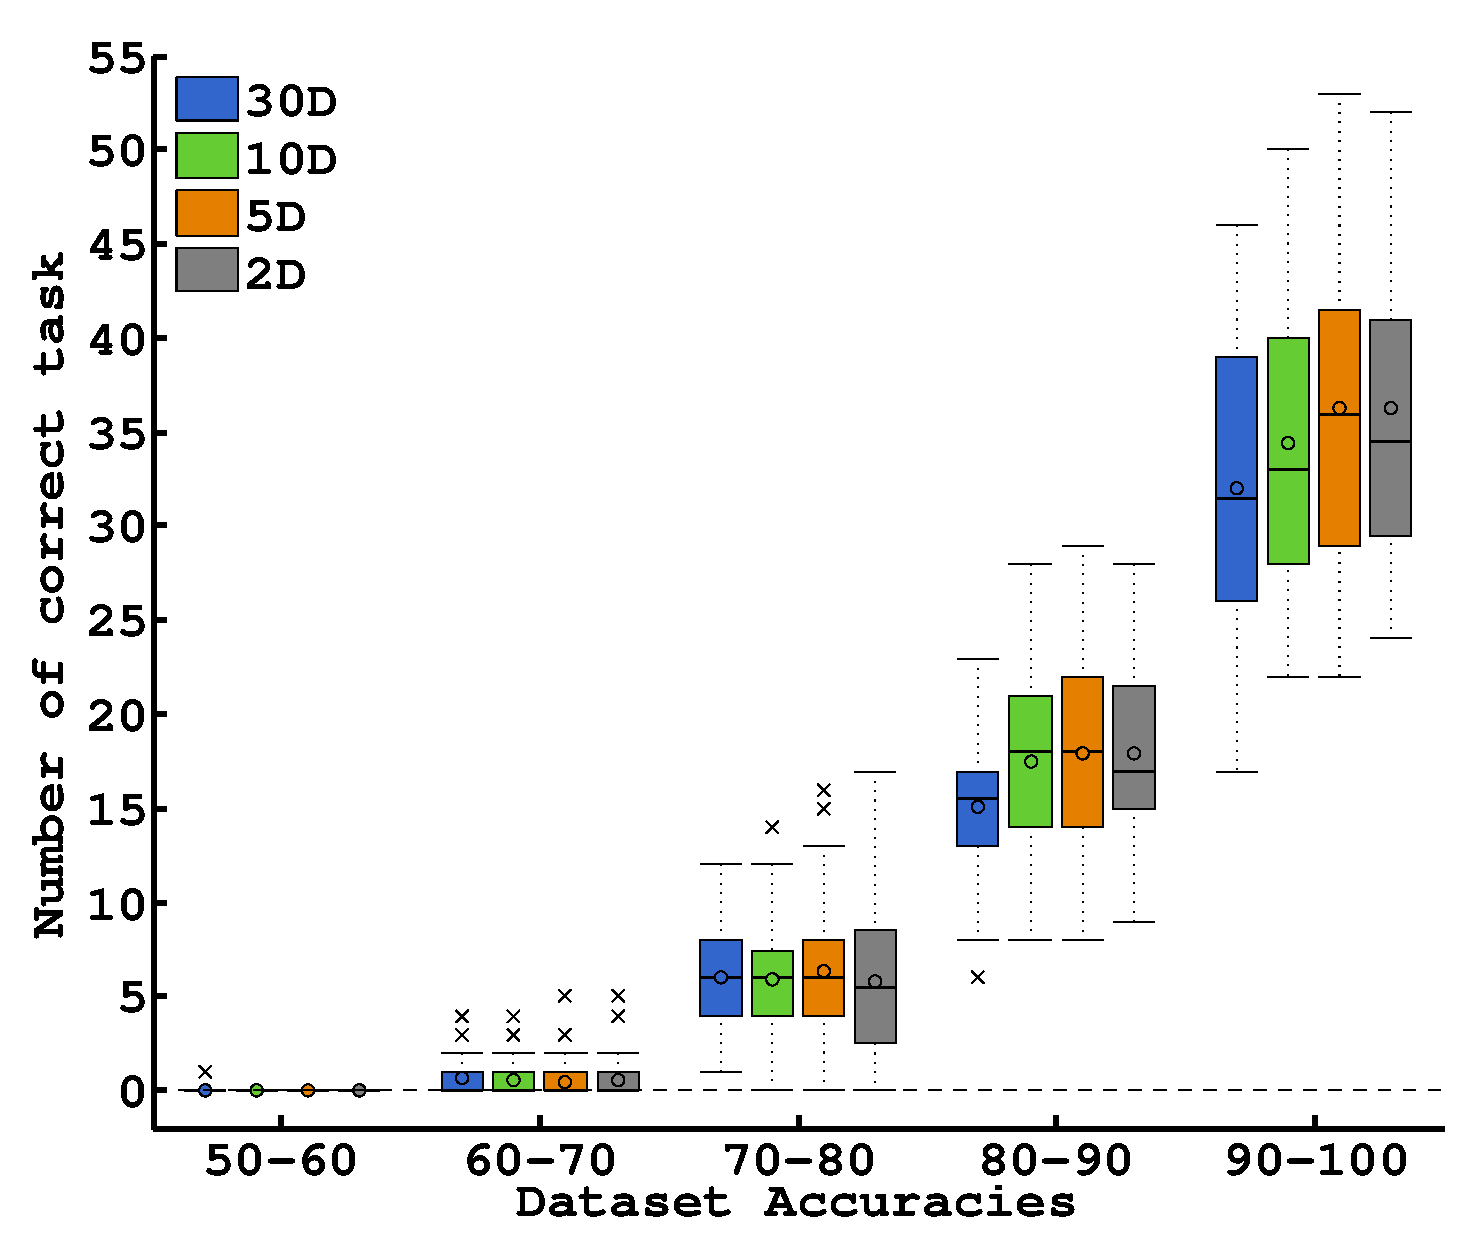
\includegraphics[width=\columnwidth]{img/plots_aaai/plot_artificial_nCorrect.eps}
% 			\caption{Quality of dataset impacts the number of task identified in 500 steps, more evidence should be collected to reach the confidence threshold.}
% 			\label{fig:nCorrectArtificial}
% \end{minipage}
% \end{figure*} 

% \begin{figure}[t]
% \centering
% 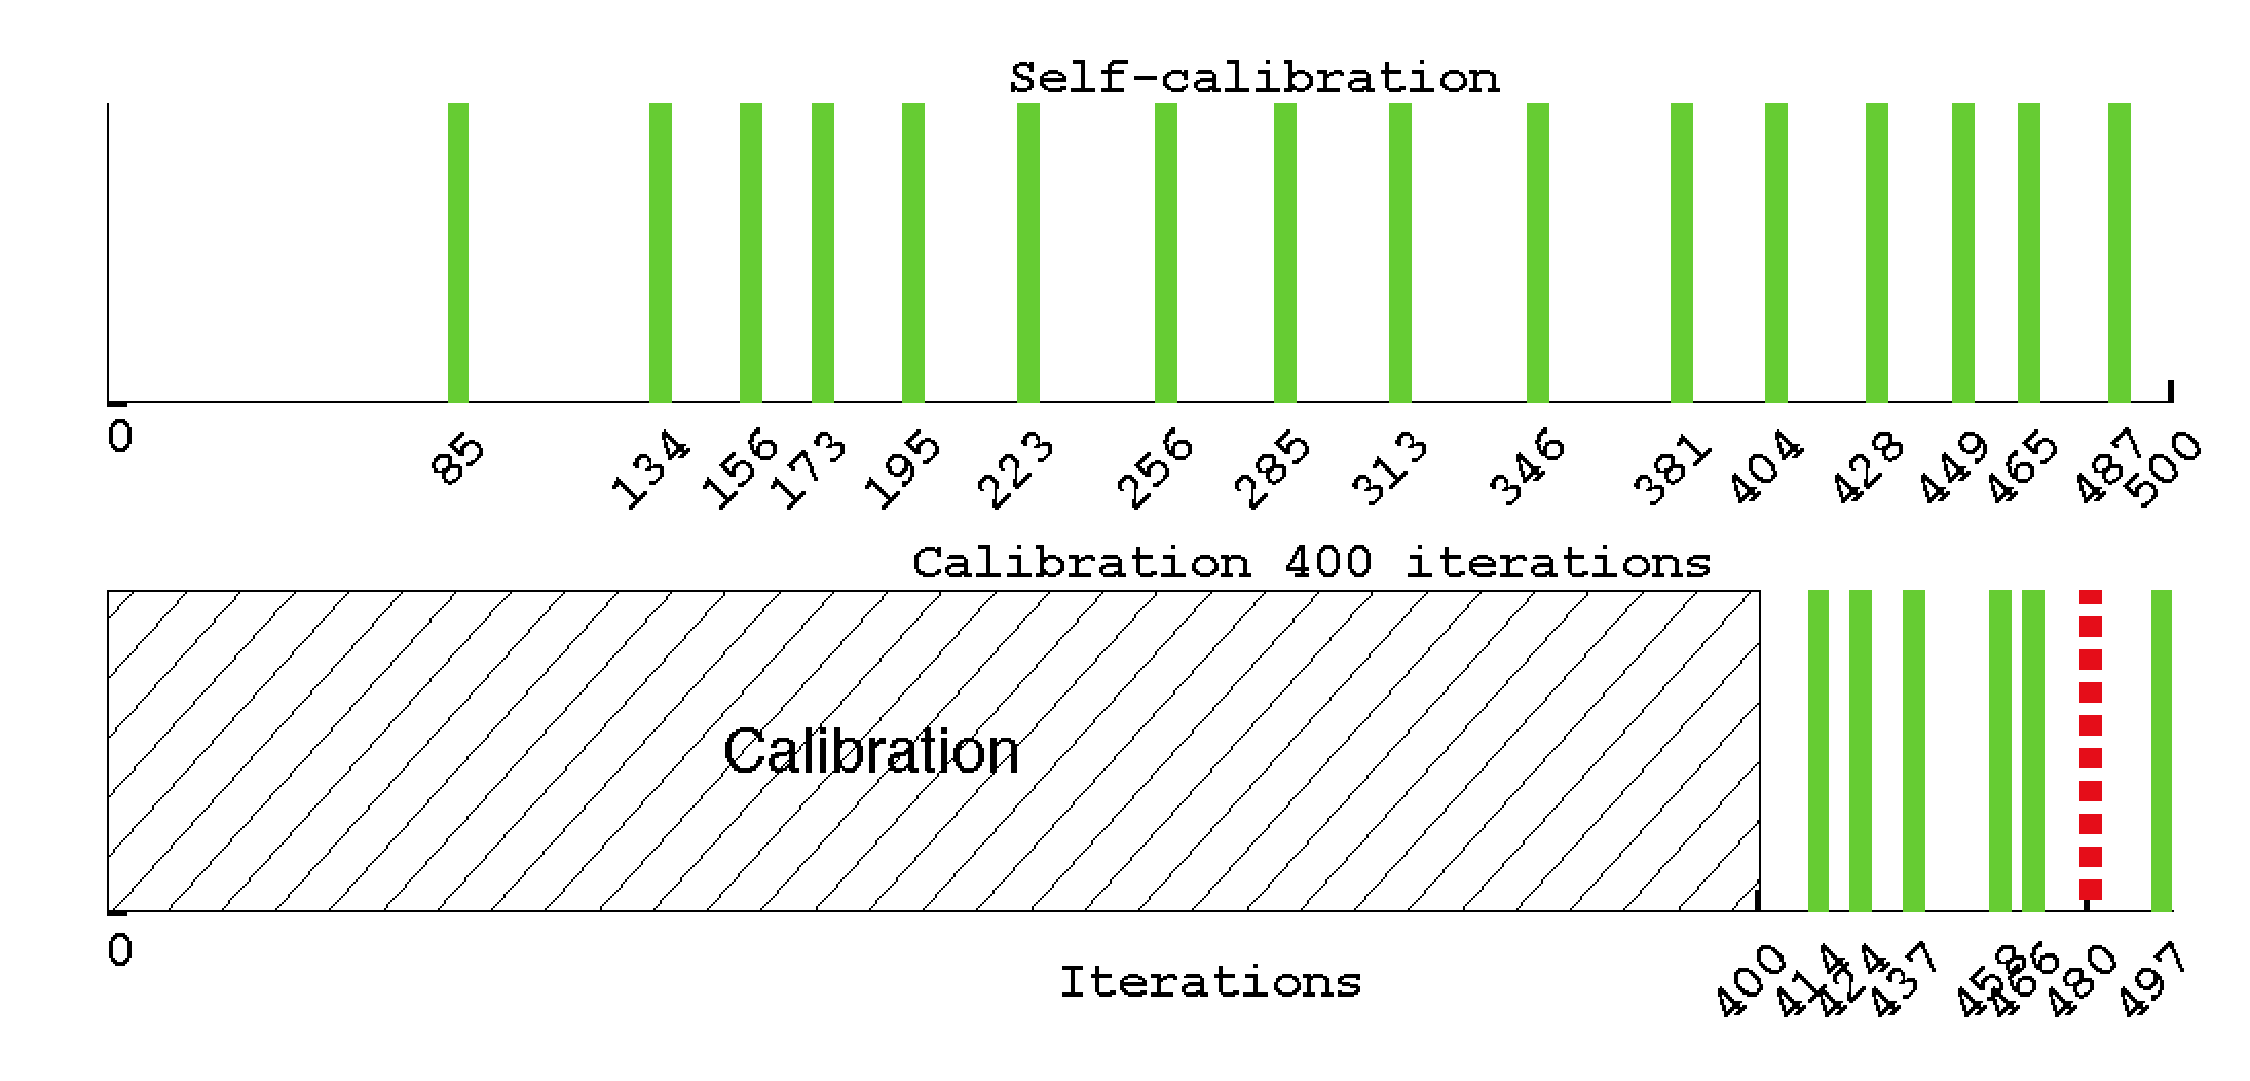
\includegraphics[width=\columnwidth]{img/plots_aaai/plot_the_aaai_sequence.eps}
% \caption{The proposed self-calibration method allow to reach a first task faster, with performance increasing with time. One run from EEG dataset of 83 percent accuracy, self-calibration versus 400 steps calibration.}
% \end{figure} 








